\documentclass[11pt]{article}

\usepackage[a4paper,left=0.5in,right=0.5in,top=0.7in,bottom=0.7in]{geometry} 
\usepackage{amsmath,amsthm,amssymb,wrapfig,graphicx}
\usepackage{todonotes}
\usepackage{eurosym}
\usepackage{wrapfig}
\usepackage{minted}
\usepackage{hyperref}
\usepackage{listings}
\usepackage{geometry}

\usepackage[parfill]{parskip}
\geometry{a4paper,left=2cm, right=2cm, top=1cm, bottom=2cm}
\renewcommand{\baselinestretch}{1.2}
\title{Assignment 1:\\ Knowledge graph construction, integration and basic querying.}
\author{Martyna Mikos - i6155316\\
Adrian Rodriguez Grillo - i6193748\\
Christian Heil - i6097391\\\\ Building and Mining Knowledge Graphs}

\begin{document}
\maketitle

\section{Mapping file}

\begin{wrapfigure}{r}{0.25\textwidth}
  \centering
   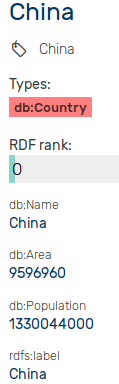
\includegraphics[width=0.15\textwidth]{images/info_box.png}
  \caption{Country information.}
  \label{fig:country_info}
 \vspace{-10mm}
\end{wrapfigure}

In this assignment, two available datasets are used in order to generate a knowledge graph that will provide a more simple and powerful way to extract information from them. These two datasets are: 

\begin{itemize}
\item The \textit{Geonames} dataset that contains information about 253 countries of the world, including the area, the population, the capital, the currency used, the top-level domain, etc. 

\item The \textit{World Bank} dataset that contains the Gross Domestic Product value from the years 1960 to 2017 of 217 countries of the world, as well of economic zones that are groups of countries (2018 is included but does not contain any value, the same as some country's values for specific years). 
\end{itemize}

\paragraph{Definition of the entities}
The first step to generate the RDF file was the definition of the triples mapping for both datasets. To do so, the logical source has to be specified, indicating the file path and the file type as well as the kind of entity that the data will form. Another aspect considered during this first phase was the selection of a shared vocabulary for the definitions in the knowledge graph, being the  \href{http://mappings.dbpedia.org/server/ontology/classes/}{DBpedia ontology} the chosen one for the provision of the definitions.

In the case of the \textit{GeoNames} dataset, the instances are defined by the \href{http://mappings.dbpedia.org/server/ontology/classes/Country}{\textit{country}} class and each one is linked to its \textit{Geonames} web page through the URI generated. The template used for the creation of the link uses the \textit{ISO} (two-character id) and \textit{Name} columns in the following way: 

{\small\texttt{http://geonames.org/countries/\{ISO\}/\{Country\}.html}}

On the other hand, the \textit{World Bank} dataset was more complicated to handle because of the lack of a specific URI to link the instances. The solution chosen involves the available World Bank API that returns the gross domestic product (GDP) for a given country and year. Therefore, the template used in the linking of the instances uses the \textit{key} of the country (three-character id) and the \textit{year} following the next structure: 

{\small\texttt{http://api.worldbank.org/v2/country/\{country/@key\}/indicator/NY.GDP.MKTP.CD?\\format=json\&date=\{year\}}}. 

In the case of the instances of the \textit{World Bank} dataset, they are defined by the \href{http://mappings.dbpedia.org/server/ontology/classes/GrossDomesticProduct}{\textit{GrossDomesticProduct}} class.

\paragraph{Adding attributes to the entities}

The second step was the selection of the attributes for the different entities created which was made taking into consideration the queries to be answered. For the first query, section (\ref{subsec:query1}), only information of the countries is required, so the population and area information was added using their respective ontology classes. In order to improve the graph, the name of the country was also added as an attribute and, more importantly, as a label, allowing a better visual search in the representation, like in figure \ref{fig:graph_example}. An example of the information that a country contains can be seen in figure \ref{fig:country_info}.

Regarding the rest of the queries (sections \ref{subsec:query2}, \ref{subsec:query3}, \ref{subsec:query4} and \ref{subsec:query5}) the GDP value is required to obtain results. Therefore, the main attributes of the \textit{Gross Domestic Product} instances are their value, the year and the country name. In this case, the label of the instances will be a string with the following template: \texttt{"GDP of \{year\}}" as can be seen in figure \ref{fig:graph_example}.

\begin{wrapfigure}{r}{0.4\textwidth}
  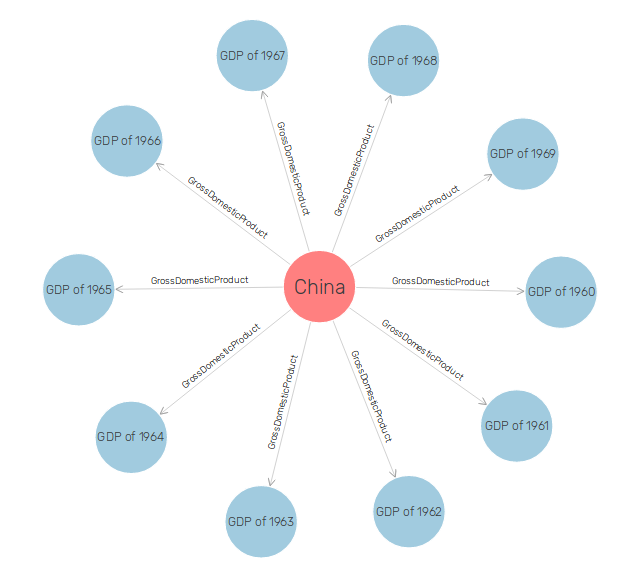
\includegraphics[width=0.4\textwidth]{images/graph-country.png}
  \caption{Example of the country with its GDP values.}
  \label{fig:graph_example}
  \vspace{-5mm}
\end{wrapfigure}

\paragraph{Countries and continents}
The fourth query (section \ref{subsec:query4}) requires an answer using the names of the continents in which different countries are situated. This information is included in the \textit{GeoNames} dataset as a column, however, it is not present in a human-readable format. A two-character id is used.

In order to improve the results of the queries, a small dataset was created including the relation between the continent identification with the full name of the continent and the string used in the DBpedia page. This dataset is included \textit{continent-codes.csv}.

This dataset defines new instances of the class \href{http://mappings.dbpedia.org/server/ontology/classes/Continent}{\textit{continent}} and its only attribute, that is also the label for the graph, is the name of the continent. Additionally, with the intention of adding more context to the dataset, we decided to link each instance with its DBpedia page so the template followed by them are:

\texttt{"http://dbpedia.org/page/\{Page\}"}

\paragraph{Datasets linking}
One of the key aspects of generating the knowledge graph is the linkage of the datasets, creating a relation between the different existent entities and allowing to make more powerful queries in a simpler way. Three entities have been described and are the ones present in the generated RDF file. Therefore, the graph contains elements of the classes \href{http://mappings.dbpedia.org/server/ontology/classes/Country}{\textit{country}}, \href{http://mappings.dbpedia.org/server/ontology/classes/Continent}{\textit{continent}} and \href{http://mappings.dbpedia.org/server/ontology/classes/GrossDomesticProduct}{\textit{GrossDomesticProduct}}. 

So as to generate this relationship among the datasets, we decided to follow the RDF specification and used the \texttt{rr:joinCondition} properties. The \href{http://mappings.dbpedia.org/server/ontology/classes/Country}{\textit{country}} entities were the chosen to contain the links to the other datasets, using the \textit{ISO3} column to join each country with its gross domestic product values and the \textit{continent} column, that contains the two-character id, with the continent where is located.

The main difficulties in this step came from the time it took to generate the triples file using the full world bank dataset (22 hours). So, in order to test that the join was done correctly we worked with a smaller file for the gross domestic product values, using an only country, however, the queries have been done in the full dataset file.

\paragraph{Final results}
As a result, the RDF triples file generated by applying the mapping files contains 92157 instances of the different classes (\href{http://mappings.dbpedia.org/server/ontology/classes/Country}{\textit{country}}, \href{http://mappings.dbpedia.org/server/ontology/classes/Continent}{\textit{continent}} and \href{http://mappings.dbpedia.org/server/ontology/classes/GrossDomesticProduct}{\textit{GrossDomesticProduct}}). 
Additionally, the execution of the last query, section \ref{subsec:query5}, adds 194 tuples containing the \href{http://mappings.dbpedia.org/server/ontology/classes/GrossDomesticProductPerCapita}{\textit{gross domestic product per capita}} of the different countries.

\section{Queries}

%list of the SPARQL queries used along with rationale for why you constructed them in the way that you did + difficulties

\subsection{Query 1\label{subsec:query1}}
Countries with a population less than 50,000 in ascending order with respect to landmass in $km^2$. This query is provided in the Appendix as code fragment \ref{listing:query1}. First 14 results are presented in Table \ref{fig:q1}. In this query filter function was used to display countries with a population below the given threshold. Results reveal an issue of missing/incorrect values in case of the first result displayed (U.S. Minor Outlying Islands) it can be seen that the population and area are 0, which in reality is a non-zero value.

\begin{figure}[H]
  \centering
   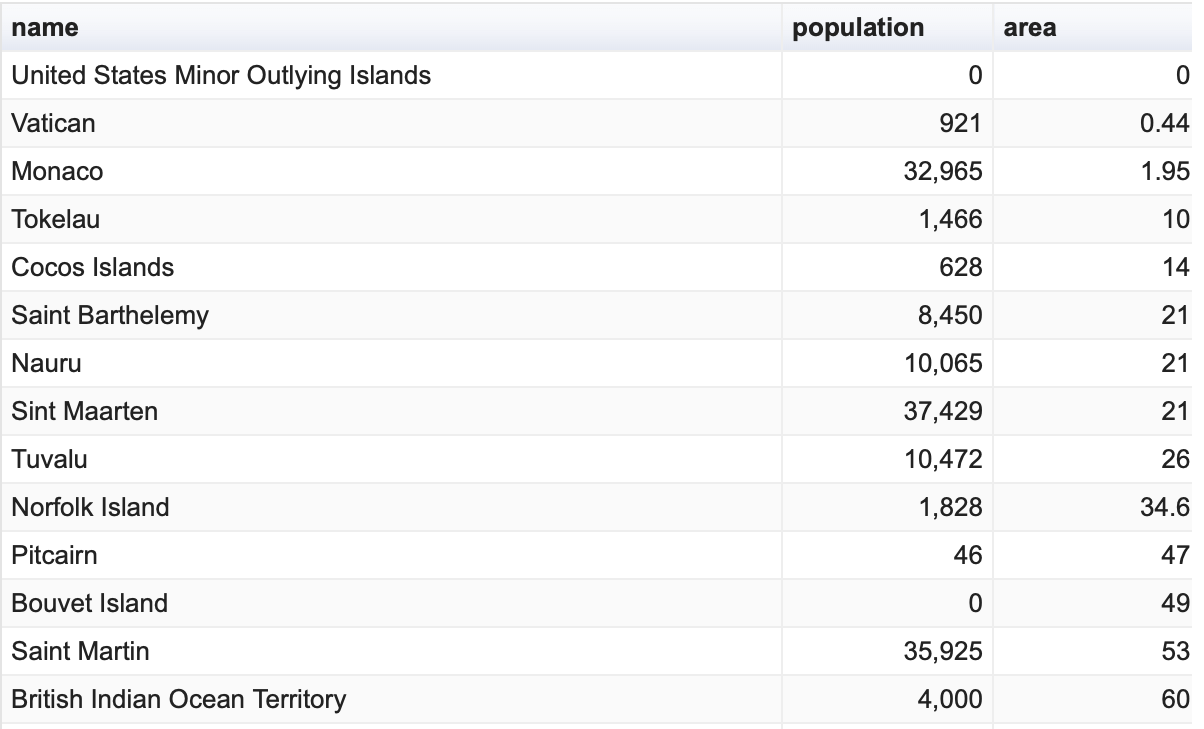
\includegraphics[width=0.8\textwidth]{results/Q1.png}
  \caption{Results for Query 1}
  \label{fig:q1}
 %\vspace{-10mm}
\end{figure}

\subsection{Query 2\label{subsec:query2}} 
Countries with the top 10 highest GDP values in 2017. Results were produced by executing the query in code fragment \ref{listing:query2} and presented in Figure \ref{fig:q2}. In the result clause \textit{?name} of the country and GDP \textit{?value} were put. Link to the country e.g. {\small\texttt{http://geonames.org/countries/US/United\%20States.html}} was replaced by its actual name and similarly the GDP value. Results were put in descending order and limited to 10. The output is coherent with the World Bank database showing the countries with the highest GDP.

\begin{figure}[H]
  \centering
   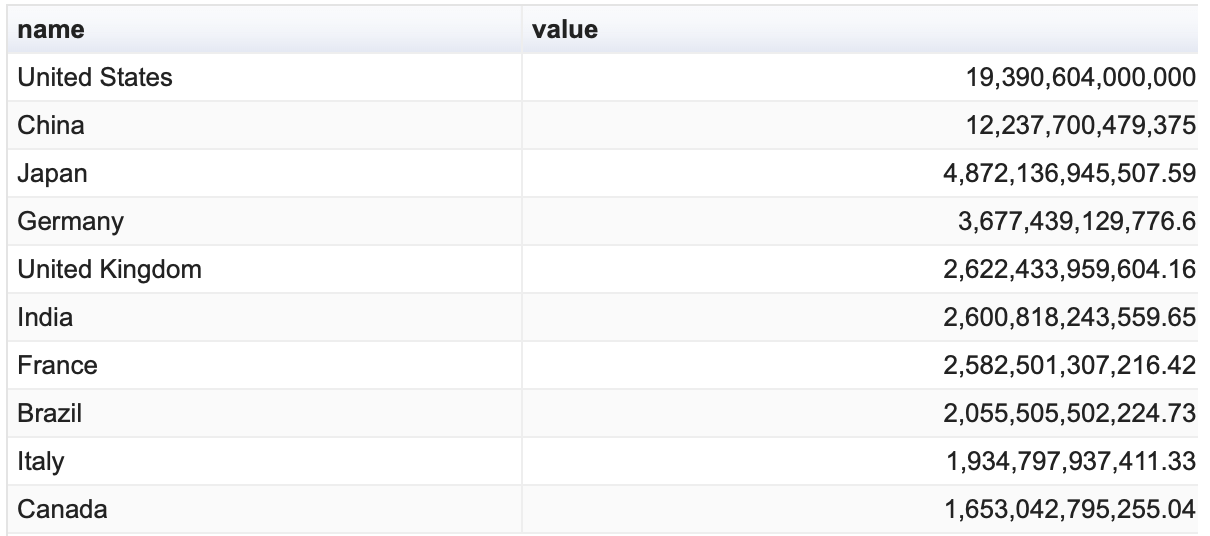
\includegraphics[width=0.8\textwidth]{results/Q2.png}
  \caption{Results for Query 2}
  \label{fig:q2}
 %\vspace{-10mm}
\end{figure}

\subsection{Query 3\label{subsec:query3}} 
Countries with the top 10 highest increases in GDP between 1960 and 2017. Code fragment \ref{listing:query3} illustrates the query. In order to produce the correct output, the GDP value for 1960 and 2017 was selected separately in the query pattern. Using \textit{BIND} function, a new variable was defined, taking the difference between the GDP values from 1960 and 2017. This value was used in the select along with the name of the country. On top of that, the value of the difference is put in descending order and using a limit clause, top 10 countries with highest GDP increase were displayed. 
 
\begin{figure}[H]
  \centering
   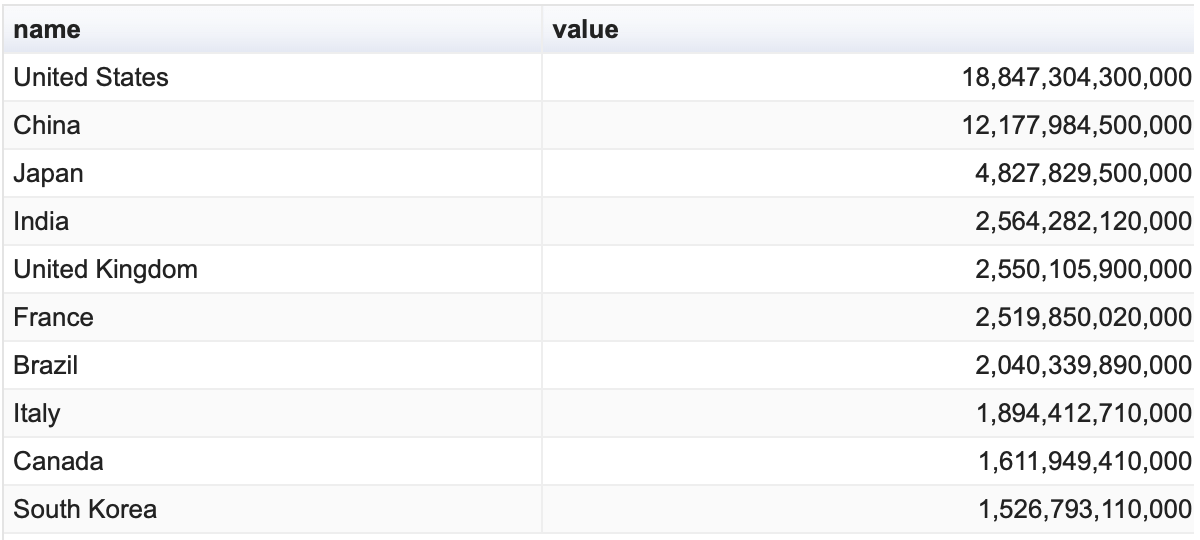
\includegraphics[width=0.8\textwidth]{results/Q3.png}
  \caption{Results for Query 3}
  \label{fig:q3}
% \vspace{-10mm}
\end{figure}

\subsection{Query 4\label{subsec:query4}} 
For each continent, The number of countries in that continent that are in the top 20 for highest increases in GDP between 1960 and 2017. The query was placed in code fragment \ref{listing:query4}. Similarly to \textit{query 3}, the GDP values for both queries were selected and a new variable being the difference between the two was created. These attributes were put in a subquery to be able to order the data in descending order by the GDP increase and by using the limit clause, select only the top 20 records. In the main result clause, the name of the continent was selected and the number of countries appearing for each continent in the top 20. 

\begin{figure}[H]
  \centering
   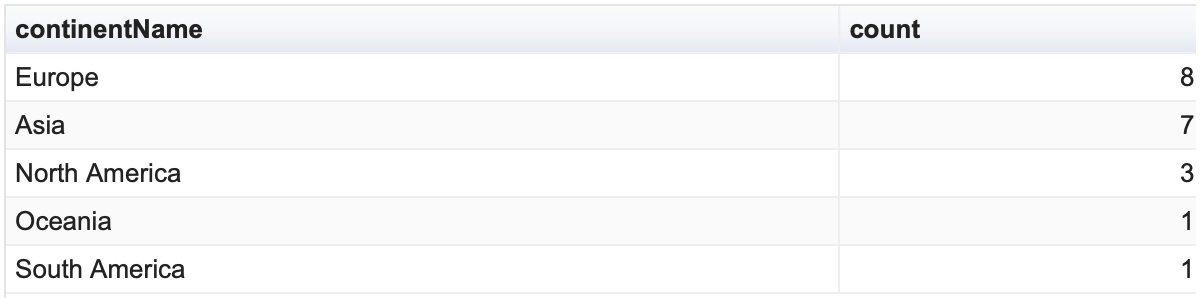
\includegraphics[width=0.8\textwidth]{results/Q4.png}
  \caption{Results for Query 4}
  \label{fig:q4}
 %\vspace{-10mm}
\end{figure}

\subsection{Query 5\label{subsec:query5}} 
Construct the triples representing the GDP per capita for each country in 2017 and directly insert them into your triplestore on GraphDB. The query was placed in the code fragment \ref{listing:query5}. Clause \textit{CONSTRUCT} was used for this exercise to build triples. A new variable called \textit{GDPperCapita} was created by dividing the value of the GDP by the population for each country in the year 2017. The query returns the subject, predicate, and object as expected.

\begin{figure}[H]
  \centering
   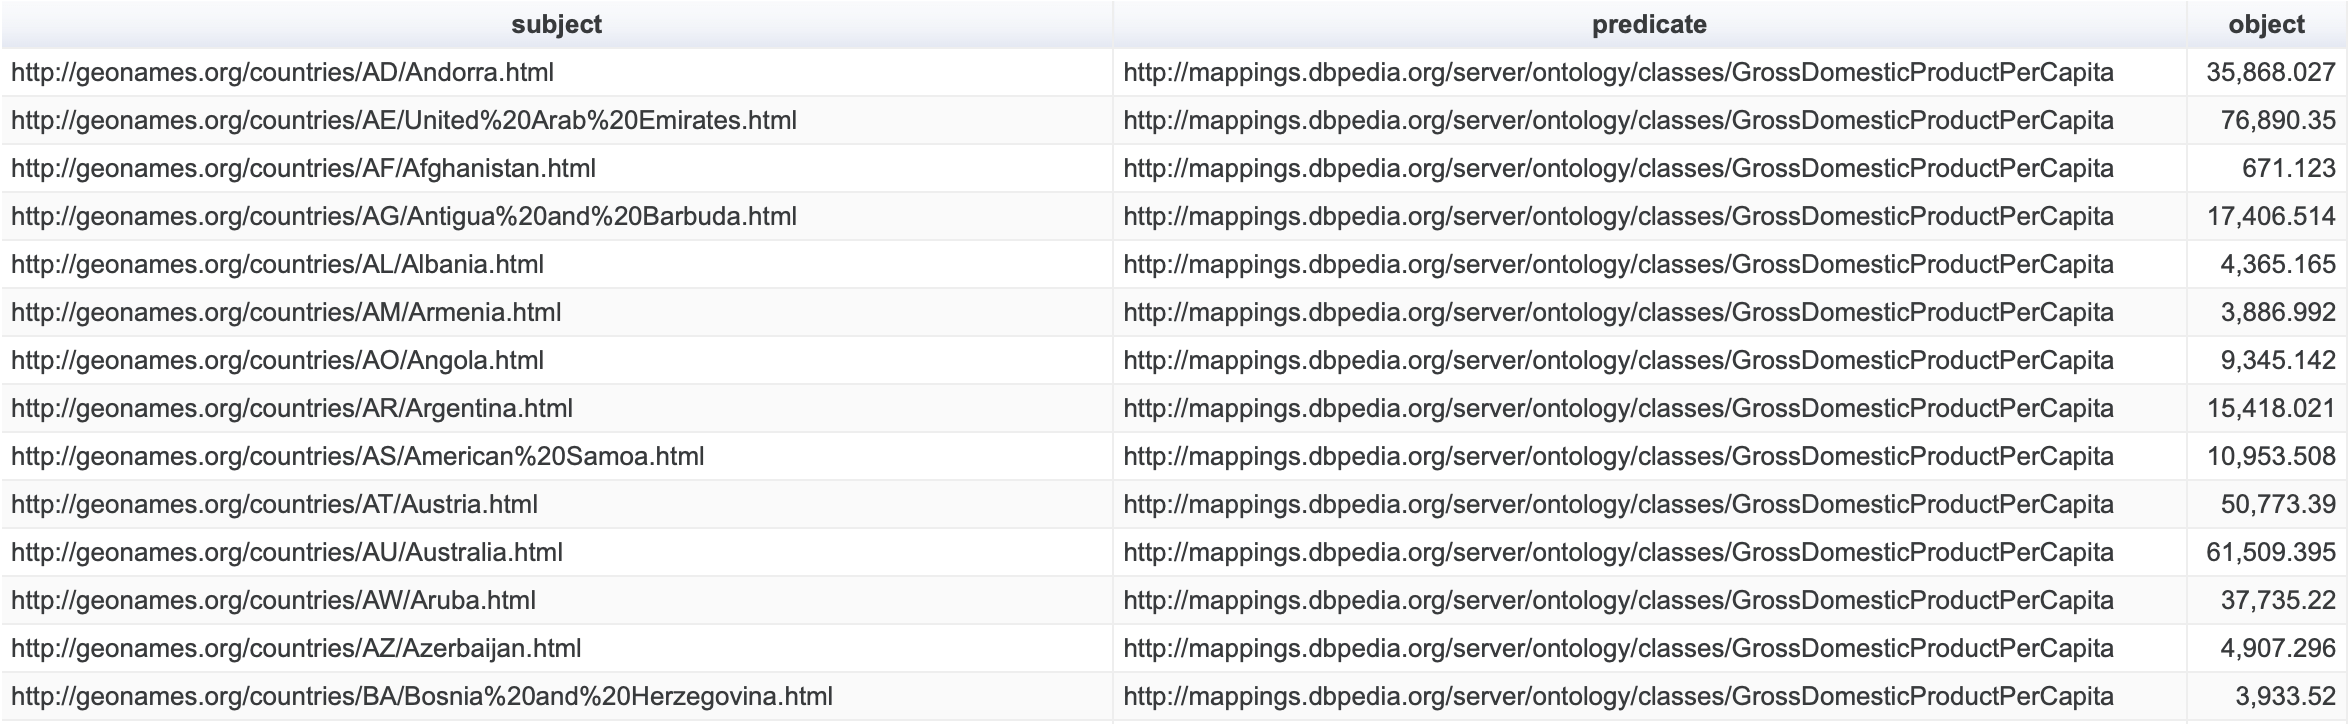
\includegraphics[width=1\textwidth]{results/Q5.png}
  \caption{Results for Query 5}
  \label{fig:q5}
 %\vspace{-10mm}
\end{figure}

\appendix
\newpage
\section{Queries}
\begin{listing}[!hbt]
\begin{minted}[frame=lines,fontsize=\footnotesize]{sparql}
PREFIX db: <http://mappings.dbpedia.org/server/ontology/classes/>

select distinct ?name ?population ?area
where { 
    ?country a db:Country .
    ?country db:Name ?name .
    ?country db:Population ?population .
    ?country db:Area ?area .
    filter (?population < 50000)
} 
order by ?area
\end{minted}
\caption{Query 1}
\label{listing:query1}
\end{listing}

\begin{listing}[!hbt]
\begin{minted}[frame=lines,fontsize=\footnotesize]{sparql}
PREFIX db: <http://mappings.dbpedia.org/server/ontology/classes/>
PREFIX rdfs: <http://www.w3.org/2000/01/rdf-schema#> 

select distinct ?name ?value
where { 
    ?country a db:Country .
    ?country db:Name ?name .
    ?country db:GrossDomesticProduct ?GDP .
    ?GDP rdfs:value ?value .
    ?GDP db:Year 2017 .
} 
order by desc (?value)
limit 10
\end{minted}
\caption{Query 2}
\label{listing:query2}
\end{listing}

\begin{listing}[!hbt]
\begin{minted}[frame=lines,fontsize=\footnotesize]{sparql}
PREFIX db: <http://mappings.dbpedia.org/server/ontology/classes/>
PREFIX rdfs: <http://www.w3.org/2000/01/rdf-schema#> 
PREFIX xsd: <http://www.w3.org/2001/XMLSchema#>

select distinct ?name ?value
where { 
    ?country a db:Country .
    ?country db:Name ?name .
    ?country db:GrossDomesticProduct ?GDP1960 .
    ?country db:GrossDomesticProduct ?GDP2017 .
    ?GDP1960 db:Year 1960 .
    ?GDP2017 db:Year 2017 .
    ?GDP1960 rdfs:value ?value1960 .
    ?GDP2017 rdfs:value ?value2017 .
    bind(xsd:float(?value2017) - xsd:float(?value1960) as ?value)
} 
order by desc (?value)
limit 10
\end{minted}
\caption{Query 3}
\label{listing:query3}
\end{listing}

\begin{listing}[!hbt]
\begin{minted}[frame=lines,fontsize=\footnotesize]{sparql}
PREFIX db: <http://mappings.dbpedia.org/server/ontology/classes/>
PREFIX rdfs: <http://www.w3.org/2000/01/rdf-schema#>
PREFIX xsd: <http://www.w3.org/2001/XMLSchema#>

select distinct ?continentName (count(distinct ?country) as  ?count)
where {
    select ?continentName ?country
    where {
        ?country a db:Country .
        ?country db:Name ?name .
        ?country db:Continent ?continent .
        ?continent db:Name ?continentName .
        ?country db:GrossDomesticProduct ?GDP1960 .
        ?country db:GrossDomesticProduct ?GDP2017 .
        ?GDP1960 db:Year 1960 .
        ?GDP2017 db:Year 2017 .
        ?GDP1960 rdfs:value ?value1960 .
        ?GDP2017 rdfs:value ?value2017 .
        bind(xsd:float(?value2017) - xsd:float(?value1960) as ?value)
    }
    order by desc (?value)
    limit 20
}
group by ?continentName
order by desc (?count)
\end{minted}
\caption{Query 4}
\label{listing:query4}
\end{listing}
    
\begin{listing}[!hbt]
\begin{minted}[frame=lines,fontsize=\footnotesize]{sparql}
PREFIX db: <http://mappings.dbpedia.org/server/ontology/classes/>
PREFIX rdfs: <http://www.w3.org/2000/01/rdf-schema#>
PREFIX xsd: <http://www.w3.org/2001/XMLSchema#>

construct {
    ?country db:GrossDomesticProductPerCapita ?GDPperCapita 
}
where {
    ?country a db:Country .    
    ?country db:GrossDomesticProduct ?GDP.
    ?country db:Population ?population .
    ?GDP rdfs:value ?GDPvalue .
    ?GDP db:Year 2017 .
    bind(xsd:float(?GDPvalue)/xsd:float(?population) as ?GDPperCapita) 
}
\end{minted}
\caption{Query 5}
\label{listing:query5}
\end{listing}




\end{document}